\documentclass[12pt,a4paper]{article} % classe article, taille 12, papier A4
\usepackage{fontspec} % permet de gérer la police

\usepackage{graphicx} % gère les images
\usepackage{array} % gère les tableaux
\usepackage{hyperref} % gère les liens
\usepackage{csquotes} % gère les citations et les guillemets

\usepackage{polyglossia} % gère l'aspect multilingue des documents
\setmainlanguage{french} % sélection de la langue principale du document

\usepackage[citestyle=authoryear-comp]{biblatex} % appel de biblatex, de nombreuses autres options disponibles
\bibliography{biblio} % appel du fichier .bib sans l'extension


% emplacement pour d'autres packages

\title{L'empaquetage des informations pour leur préservation à long terme} % le titre du document
\author{Tommy De Ganck} % son auteur
\date{8 janvier 2024} % la date


%% début du document

\begin{document} % début du corps du texte

\maketitle % affiche le titre, l'auteur et la date
	

\section{Introduction} % présentation de la pertinence, de l'objectif et de la structure de l'article
Le présent travail s'intéresse aux formats d'empaquetage des informations pour leur préservation à long terme. Dans ce contexte, l'empaquetage consiste à conditionner le contenu à archiver avec les métadonnées qui s'y rapportent. Pour qu'un tel paquet soit identifiable, lisible et donc utilisable, il est nécessaire de décrire la structure du paquet ainsi que les liens entre le contenu archivé (et ses différents éléments), d'une part, et les métadonnées qui leur sont associées, d'autre part. 

L'empaquetage est un élément clé de tout projet d'archivage électronique. En effet, la conservation pérenne des contenus implique de les documenter suffisamment afin d'être capable d'en assurer une gestion optimale dans le temps, d'y effectuer des recherches et d'en permettre la consultation (par virtualisation notamment). Or, les contenus à conserver sont non seulement de plus en plus nombreux, mais également de plus en plus complexes. L'empaquetage des informations à archiver doit donc répondre au double défi d'un encapsulage performant (qui décrit et relie tous les éléments utiles d'une façon structurée) et économique (qui évite les redondances sans compromettre la pérennité des l'accès aux ressources nécessaires). 

Cette question est abordée ici dans le contexte de l'\textit{Open Archival Information System} (OAIS), que l'on peut traduire par "Système ouvert d'archivage d'information". Deux standards d'empaquetage basé sur l'\textit{Extensible Markup Language} (XML) sont présentés et comparés : le \textit{Metadata Encoding and Transmission Standard} (METS) et le \textit{XML Formatted Data Unit} (XFDU). 

Après un bref historique de l'OAIS et des initiatives prises sur le plan international pour organiser son implémentation, j'introduis de façon synthétique le système décrit dans l'OAIS et plus spécifiquement la notion de "paquet d'information". Je présente ensuite successivement les standards METS et XFDU avant d'en esquisser une comparaison en guise de conclusion. 

\section{Contexte} % explication du contexte historique de l'OAIS et des initiatives liées à l'implémentation sur le plan international
\subsection{OAIS}
Le cadre méthodologique général actuellement reconnu et utilisé internationalement pour l'archivage et à la préservation à long terme de documents numériques est l'\textit{Open Archival Information System} (OAIS). OAIS est un modèle conceptuel destiné à la gestion, à . Il a été élaboré par le \textit{Consultative Committee for Space Data Systems} (CCSDS), un organisme regroupant les principales agences spatiales du monde. Il a été publié pour la première fois en 2002 comme standard CCSDS. Le standard est rapidement enregistré entant que norme ISO (en 2003\footnote{sous la référence 14721:2003}). La norme ISO a fait l'objet d'une révision en 2012\footnote{sous la référence 14721:2012}.

L'OAIS définit les principes, les concepts, les responsabilités et les fonctions d'un système d'archivage numérique capable de préserver l'information sur le long terme. Les auteurs de la norme insistent sur le fait qu'il n'est pas possible de garantir une conservation éternelle, même si le but est de viser une préservation aussi longue que possible. Il faut dès lors comprendre le "long terme" comme une durée suffisamment longue que pour être soumis à l'impact des évolutions technologiques et des besoins des utilisateurs. OAIS est un modèle conceptuel général et ne fournit pas de spécifications techniques. Le modèle OAIS a plutôt pour vocation de fournir des lignes directrices et des bonnes pratiques pour concevoir et mettre en œuvre un système d'archivage numérique conforme aux exigences de pérennisation. Il propose un vocabulaire commun et un cadre théorique pour faciliter les échanges entre les différents acteurs impliqués\footnote{Les informations d'ordre général sur le modèle OAIS sont aisément et librement accessibles en ligne. Vous pouvez consulter \href{https://www.fr.wikipedia.org/wiki/Open_Archival_Information_System}{la fiche de Wikipedia dédiée à OAIS} et \href{http://www.oais.info/}{site d'information officiel sur le modèle}}.

Le cadre théorique du modèle OAIS se compose essentiellement de deux types de modèles tous les deux détaillés au sein de la norme : le modèle d'information et le modèle fonctionnel. Le modèle d'information décrit la structure et le contenu des informations archivées et créée à cette occasion une nomenclature spécifique (j'y reviens au point suivant). Il définit également les métadonnées associées à ces objets, qui permettent de les identifier, de les décrire, de les gérer et de les rendre accessibles. Le modèle fonctionnel décrit les activités et les services que doit assurer un système d'archivage numérique, regroupés en six fonctions principales : ingestion, gestion des données archivistiques, préservation, gestion de l'administration, gestion du planning et accès.
\subsection{Normes associées}
Largement accepté et utilisé  par diverses organisations et disciplines, tant nationales qu'internationales, OAIS constitue aujourd'hui une référence incontournable pour l'archivage numérique, mais reste insuffisante pour assurer sa mise en oeuvre. C'est pourquoi le modèle OAIS a servi de base à l'élaboration d'autres normes et standards associés qui sont autant de briques supplémentaires indispensables pour implémenter ses principes dans un projet concret d'archivage électronique. Ces normes et standards sont d'ailleurs renseignés en tant que tel au sein de la norme\footnote{Voyez \href{https://public.ccsds.org/Pubs/650x0m2(F).pdf}{les pratiques recommandées}} et une liste de ceux-ci est régulièrement mise à jour sur le site d'information officiel au sein d'un \href{http://www.oais.info/standards-process/oais-roadmap-and-related-standards/}{"parcours"} qui les présente dans l'ordre utile au niveau de la mise en oeuvre (depuis la préparation des données à ingérer jusqu'à la certification du système d'archivage mis en place).Une série d'étape au sein de ce parcours n'ont pas encore de standard spécifique disponible, ce qui met en lumière que l'effort de normalisation ne couvre pas encore tous les aspects de l'implémentation.

Logiquement, les normes et standards déjà mis au point concernent les aspects liés aux premières étapes de la mise en oeuvre : la préparation et l'ingestion des données et métadonnées. 

Dès 2003, soit à peine un an après la parution du modèle OAIS, le CCSDS élabore la norme PAIMAS (\textit{The producer-Archive Interface Methodology Abstract Standard}. PAIMAS est un guide méthodologique qui définit les différentes phases de la préparation du transfert d'information (\textit{ingest}). Son objectif est de faciliter la bonne gestion des projets et d'améliorer la qualité des données archivées en établissant un cadre d'interaction prédéfini entre les producteurs (des données à archiver) et les archives (responsables de l'archivage). PAIMAS définit quatre étapes et liste pour chaque d'elle les questions à résoudre, les choix à effectuer et les informations à collecter pour pouvoir passer à la suivante et finalement effectuer le transfert. PAIMAS vise à diminuer les pertes en qualité des données et en ressources investies en augmentant la prévisibilité et l'homogénéité des procédures : \enquote{\textit{Our experience of archiving, and an analysis carried out on many practical cases, showed the existence of recurrent difficulties between a Producer and an Archive [...]. Typical problems are delivered information is incomplete or it doesn't correspond to what is expected, errors in archived data are often detected late in the process, modifications are not properly managed, and planning is not respected. [...] [Another problem is that] the archives consistently redefine the interface methodology regardless of the fact that the process is more or less equivalent from one project to the other. These actions led to lower archived information quality, duplicated work, lack of generality, and resulted in higher costs. The PAIMAS was developed to address these issues}}\autocite{Garrett2004}.

Complémentaire à PAIMAS, la norme \textit{Producer-Archive Interface Specification} (PAIS) permet sa mise en oeuvre technique et modélise la forme des paquets échangés et leur contenu. Une version préliminaire de la norme est publiée dès 2006 par le CCSDS\footnote{PAIS devient une norme ISO en 2015 sous la référence ISO 20104:2015; une révision a eu lieu en 2023}. Pour encourager et faciliter son adoption, un document explicatif contenant des exemples complets est publié en 2016\footnote{\href{https://public.ccsds.org/Pubs/651x2g1.pdf}{Ce document est accessible en ligne}}.Les modèles d'empaquetage décrits par PAIS reposent sur l'usage du XFDU, élaboré également par le \href{https://public.ccsds.org/Pubs/661x0b1.pdf}{CCSDS en 2008}. La norme XFDU fournit un ensemble de catégories et de classifications de métadonnées prédéfinies qui caractérisent le contenu, le contexte, la provenance, la qualité et la préservation des données et des métadonnées dans le paquet.

On voit donc que le CCSDS a élaboré un ensemble de normes ayant vocation à fonctionner ensemble pour mettre en oeuvre OAIS. Cependant, d'autres organismes ont également élaboré des normes compatibles. 

La plus couramment citée dans la littérature européennes est METS. Cette norme a été élaboré dès 2001, soit avant la publication du modèle OAIS, par un groupe d'experts issus de la communauté de la Librairie du Congrès. Dès 2006, les Archives de France démarre l'élaboration d'un modèle d'échange de données pour l'archivage. Ce travail donne lieu à la publication en 2014 de la norme MEDONA (Modélisation des échanges de données pour l'archivage)\footnote{norme AFNOR NF Z 44-022}.MEDONA est plus tard adaptée pour permettre son adoption à l'international et en dehors du secteur public et paraît en 2017 en tant que "\textit{Data exchange protocol for interoperability and preservation} (DEPIP)\footnote{sous la référence ISO 20614:2017}.Contrairement aux normes PAIMAS et PAIS (et à son outil associé XDFU), MEDONA (et DEPIP) ne se focalise pas uniquement sur le processus d'ingestion des données, mais couvre différentes situations d'échange de données (transfert, livraison, destruction, archivage et stockage) et définit des scénarios d'usage. La norme inclut des diagrammes d'activité, des modèles de données en UML et des schémas XML pour l'échange de données. Contrairement à PAIS, MODENA ne spécifie pas comment et avec quel format d''empaquetage les objets numériques doivent être transférés avec leurs métadonnées\autocite{grimouard_data_2014}. 


\section{Le concept de "paquet d'information"}
Avant de plonger plus en détail sur l'usage de METS et de XFDU pour l'empaquetage des information à archiver, il est nécessaire de définir la notion de "paquet d'information" et de la situer au sein du modèle de données décrit dans l'OAIS. 

L'empaquetage d'information consiste à établir des liens entre un ensemble de données et les métadonnées qui les décrivent. L'empaquetage est important pour assurer une interprétation et une exploitation des données à la fois par les humains et les machines. Le "paquet d'information" est un des concepts clés du modèle OAIS. Il s'agit d'une entité logique qui regroupe les données à archiver et les métadonnées associées, permettant ainsi de garantir leur intelligibilité, leur authenticité, leur accessibilité et leur pérennité. Les paquets d'information sont en quelques sorte la "matière première" du système puisque c'est grâce à et sur ces paquets d'informations que seront appliqués les différentes fonctionnalités du système d'archivage. 

Le modèle de données décrit dans l'OAIS établit une distinction entre les différents paquets d'information selon leur statut au sein du processus de gestion archivistique. Il existe ainsi trois types de paquets d'informations  :
- Le paquet d'informations de soumission (SIP) : il correspond à l'objet numérique fourni par le producteur à l'archive, accompagné des métadonnées nécessaires à son identification, sa description, sa validation et son ingestion.
- Le paquet d'informations archivistiques (AIP) : il correspond à l'objet numérique stocké dans l'archive, après avoir été transformé et enrichi par le processus d'ingestion. Il contient les métadonnées descriptives, techniques, administratives et de préservation relatives aux données archivées.
- Le paquet d'informations de diffusion (DIP) : il correspond à l'objet numérique fourni par l'archive à l'utilisateur, après avoir été extrait et adapté par le processus d'accès. Il contient les métadonnées nécessaires à la compréhension et à l'utilisation des données diffusées (\cite{giaretta_advanced_2011}).

La norme OAIS ne fournit une description détaillée que pour l'AIP. C'est en effet l'AIP qui est au centre des opérations de l'OAIS. 
L'image ci-dessous présente l'ensemble des éléments qu'un AIP inclut\footnote{Image provenant de \cite{giaretta_advanced_2011}, p.62}. 

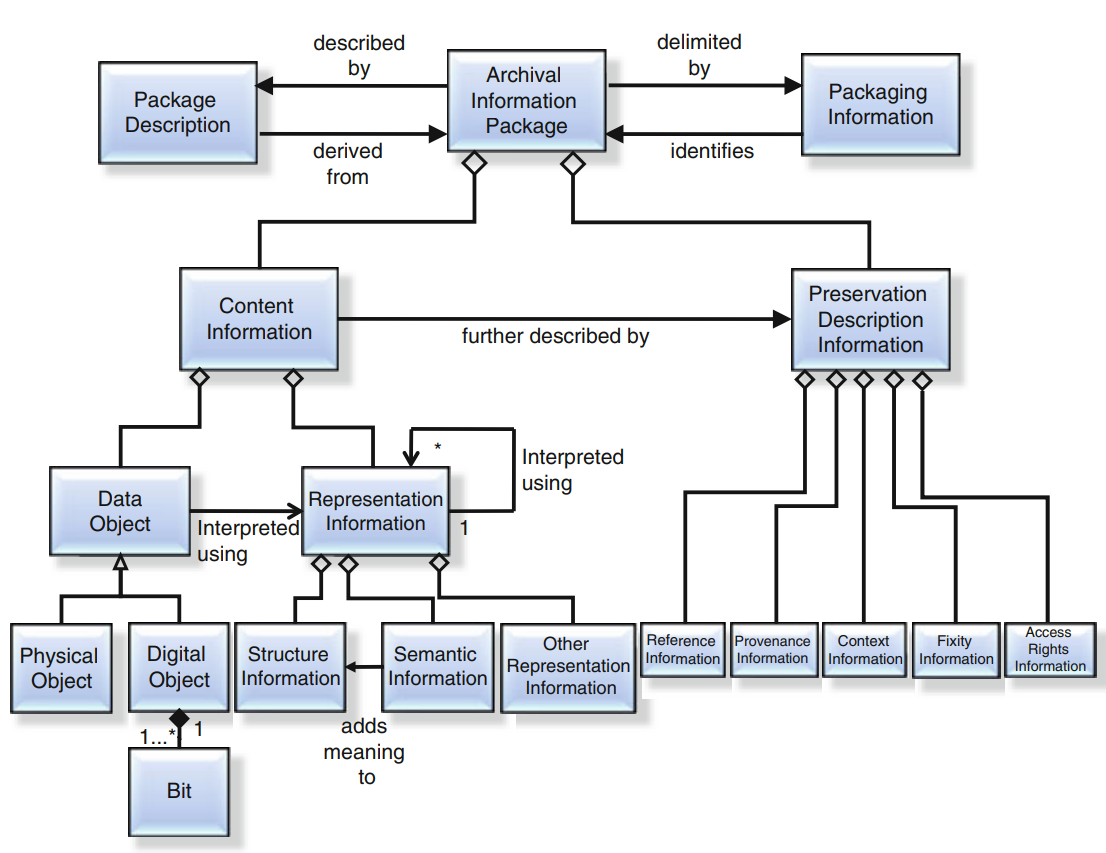
\includegraphics[width=0.95\textwidth]{Full_AIP_package}.

D'un point de vue logique, chaque paquet d'information est décrit et identifié en tant qu'ensemble particulier (par le\textit{Package Description}. Son contenu est constitué de deux grandes catégories de données : le CDO ou \textit{Content Data Object}, qui regroupe les données à préserver, et le PDI ou \textit{Preservation Description Information}, qui rassemble les informations nécessaires pour assurer la conservation du CDO. Chacun est son tour constitué de différents éléments. Le CDO contient le \textit{data object}, qui est le contenu informationnel que l'on souhaite conserver, et l'information de représentation, qui regroupe les informations nécessaire à l'interprétation correcte du \textit{data object}. Le PDI contient cinq catégories qui permettent de référencer les données, de connaître leur provenance, leur contexte, leur intégrité et les règles d'accès qui doivent être respectées. Étant donné la complexité et la multiplicité des informations potentiellement contenues dans un paquet, il est essentiel d'identifier ses différentes parties et d'établir des liens entre celles-ci. 


\section{Formats d'empaquetage}
Les formats METS et XFDU sont deux manières différentes d'utiliser des schémas XML afin de structurer et décrire des paquets d'information. 
\subsection{METS}
METS est créé en 2001 pour encoder les métadonnées descriptives, administratives et structurelles en utilisant l'\textit{ Extensible Markup Language Schema} (XSD). Le projet, développé par la \textit{Digital Library Federation}, est né de la volonté d'étendre son prédécesseur, le projet \textit {Making of America II} (MOA2), qui avait élaboré un \textit{Document Type Definition} (DTD) pour l'encodage des métadonnées, au moment où une version préliminaire de l'OAIS était parue. METS est alors mis au point pour créer les paquets d'information décrits par OAIS (\cite{cantara_mets_2005}, p.236-239). 

METS est composé de sept sections possibles. Après l'en-tête METS (METS Header), qui contient des informations générales sur le document (comme le créateur, le titre, le type, la date, l'identifiant, etc.), on retrouve la racine du schéma qui est le document METS lui-même et qui contient six catégories de métadonnées décrivant le paquet :
\begin{enumerate}
    \item La section descriptive (\textit{Descriptive Section}) décrit les caractéristiques de l'objet numérique, comme son contenu, sa structure, son origine, ses droits, etc. Elle peut utiliser différents schémas de métadonnées, comme Dublin Core, MODS, PREMIS, etc.
    \item La section administrative (\textit{Administrative Section}) fournit des informations techniques sur l'objet numérique, comme son format, sa taille, sa résolution, son empreinte numérique, etc. Elle peut également inclure des informations sur la provenance, la conservation, les droits d'accès, etc.
    \item Le manifeste des fichiers (\textit{File Section}) liste tous les fichiers qui font partie de l'objet numérique. Il indique leur nom, leur emplacement, leur identifiant et leur type MIME.
    \item La section de structuration (\textit{Structural Section}) définit la structure logique et physique de l'objet numérique. Elle indique comment les fichiers qui composent l'objet sont organisés et reliés entre eux. Elle peut utiliser différents types de structures, comme hiérarchique, séquentielle, parallèle, etc.
    \item La section de structuration des liens est un complément à la carte structurelle qui nous permet d'enregistrer les liens qui traversent sa structure hiérarchique.
    \item La section comportementale (\textit{Behavioral Section}) spécifie les actions ou les services associés à l'objet numérique. Elle peut définir des comportements internes ou externes, comme l'affichage, la lecture, la transformation, la validation, etc.
\end{enumerate}

METS a été largement adopté pour l'archivage. Son principe est flexible puisqu'il permet l'intégration de toute sorte d''autres standards XML à travers l'usage d'extensions, qui sont intégrées à sa structure ou référencées. Son architecture est conçue pour permettre un empaquetage efficace des informations, en intégrant des catégories de métadonnées clairement distinctes mais bien reliées entre elles par un système d'identifiants et de pointeurs internes qui constituent ensemble un système efficace de représentation des liens entre les métadonnées d'objets numériques complexes \autocite{gartner_metadata_2021}. 

La flexibilité de METS est l'une des principales raisons de son succès selon Katherine Ralson. En effet, étant donné les coûts induits par l'adoption d'un nouveau standard de métadonnées est très élevé et METS permet d'implémenter une stratégie de préservation numérique qui intègre et tire parti de l'ensemble des métadonnées déjà utilisées dans les systèmes de productions et/ou de description des contenus \autocite{ralson_mets_2013}. 


\subsection{XFDU}
La norme XFDU spécifie comment regrouper les données et les métadonnées pour faciliter le transfert et l'archivage des informations. Conforme au modèle OAIS, XFDU a été adopté adoptée par plusieurs agences spatiales, telles que l'ESA (Agence spatiale européenne). 

XFDU fournit un ensemble de catégories et de classifications de métadonnées prédéfinies qui caractérisent le contenu, le contexte, la provenance, la qualité et la préservation des données et des métadonnées du paquet d'information. Il permet de créer des structures hiérarchiques qui lient les données et les métadonnées associées, ainsi que de définir des règles de validation et de transformation. 

Un empaquetage avec XFDU est composé de deux parties principales : le manifeste et le contenu. Le manifeste est un fichier XML qui décrit les métadonnées, les relations et les références des données contenues dans l'empaquetage. Le manifeste suit un schéma XSD qui définit les éléments et les attributs autorisés. Le manifeste contient des informations telles que l'identifiant, le titre, la date, le créateur, le format, la taille, le \textit{checksum} et la localisation des données. Le contenu est l'ensemble des données numériques qui sont empaquetées avec le manifeste. Le contenu peut être de différents types, tels que des fichiers binaires, des fichiers XML, des images, des vidéos, des sons, etc. Le contenu est référencé par le manifeste à travers des URI (\textit{Uniform Resource Identifier}) \autocite{dunckley_using_2010}.

Tous les éléments de contenus dans le paquet d'information sont référencés par le manifeste, qui est constitué de cinq sections : 
\begin{enumerate}
\item L'entête (\textit{Header}) contient des informations sur le nom, la version, la date et l'identifiant du manifeste, ainsi que sur l'organisation ou l'entité qui l'a créé.
\item La section \textit{Information Package Map} décrit la structure hiérarchique du paquet de données, en utilisant des éléments appelés Data Object Pointer pour référencer les objets de données inclus dans le paquet ou accessibles par des liens externes.
\item La section \textit{Data Object} contient les objets de données eux-mêmes, sous forme de séquences d'octets, ou des références à des sources externes où les objets de données peuvent être trouvés.
\item La section \textit{Metadata} contient des métadonnées associées aux objets de données ou au paquet dans son ensemble, sous forme d'éléments XML ou de références à des schémas externes.
\item La section \textit{Behavior} décrit le comportement attendu du paquet de données, c'est-à-dire les actions ou les opérations qui peuvent être effectuées sur le paquet ou ses composants, en utilisant des pointeurs pour référencer des scripts, des programmes ou des services externes.
\end{enumerate}

XFDU n'a pas encore été largement utilisé par la communauté internationale dans des projets de préservation numérique. La littérature disponible (\autocite{dunckley_using_2010, giaretta_advanced_2011} se fonde sur l'exemple de CASPAR (\textit{Cultural, Artistic and Scientific knowledge for Preservation, Access and Retrieval}), un projet financé par la Commission européenne qui s'est déroulé de 2006 à 2009. Son l'objectif était de développer des méthodes et des outils pour préserver et accéder aux données numériques culturelles, artistiques et scientifiques \footnote{\href{https://www.casparpreserves.eu/}{Voyez le site du projet}}.

Au sein du projet CASPAR, XFDU était l'un des trois conteneurs envisagés pour empaqueter les informations. Les deux autres étaient METS et MPEGS-21. XFDU a été choisi car au début du projet, METS n'était pas encore complètement adapté au modèle OAIS, et les partenaires du projet n'avait pas d'expérience passées avec METS contrairement à XFDU qui avait déjà été utilisé par l'Agence spatiale européenne (\cite{dunckley_using_2010}, p. 5). Par ailleurs, le XFDU permet d'inclure des information additionnelles si nécessaire afin de répondre à des besoins spécifiques sans pour autant renoncer à la cohérence de l'ensemble et aux principes de la standardisation (\cite{giaretta_advanced_2011}, p. 194).

\section{Conclusion}
METS et XFDU sont deux usages des schémas XML pour formaliser l'empaquetage de paquets d'information dans le cadre de la conservation à long terme. METS a été plus largement adopté que XFDU dans ce contexte. Ce dernier est surtout connu dans le cadre de la préservation des données spatiales. La popularité de METS tient à son architecture flexible qui rend facile son adoption car il intègre facilement et se combine bien avec les autres standards déjà adoptés par la communauté professionnelle. XFDU de son côté, répond particulièrement aux normes de l'OAIS, mais est davantage adapté à des projets où le besoin en spécialisation est élevé, là où METS permet un usage générique et donc une implémentation dans des projets et plateformes qui agrègent des contenus d'origine et de nature très variées (comme \textit{Europeana}).

%% bibliographie
\printbibliography

\end{document}